% !TeX encoding = UTF-8
% !TeX spellcheck = en_US
\documentclass[11pt, a4paper]{article}
\usepackage{graphicx} 
\usepackage[export]{adjustbox}
\usepackage[left=2cm,right=2cm,top=2cm,bottom=2cm]{geometry} 
\usepackage{array, booktabs, longtable}
\usepackage{url}
\usepackage{hyperref}
\usepackage{xparse}
\usepackage{array}
\newcolumntype{C}[1]{>{\centering\arraybackslash}p{#1}}
\usepackage{fp}
\usepackage[usenames,dvipsnames]{xcolor}



% The title of the current document to be produced.
\NewDocumentCommand{\doctitle}{}{Sillabo del Corso}
\NewDocumentCommand{\materialedidattico}{o}{%
    \IfNoValueTF{#1}
        {\redtext{\textbf{Materiale didattico~}}}
        {\redtext{\textbf{Materiale didattico:~} #1}}}
\NewDocumentCommand{\argomento}{o}{%
    \IfNoValueTF{#1}
        {\bluetext{\textbf{Argomento~}}}
        {\bluetext{\textbf{Argomento:~} #1}}}
\NewDocumentCommand{\dataeora}{o}{%
    \IfNoValueTF{#1}
        {\textcolor{ForestGreen}{\textbf{Data e ora~}}}
        {\textcolor{ForestGreen}{\textbf{Data e ora:~} #1}}}

%
\setlength{\unitlength}{1in}
\renewcommand{\arraystretch}{2}

%------------------------------------------------------------
% Import commands for both teacher and course information.  | 
% NOTE: Change your teacher and course info in these files. |
%------>------>------>------>------>------>------>------>-->|
%% ==================================
%% ===== Teacher info             ===
%% ==================================
%%
\newcommand{\instructor}{Giancarlo Succi}
\newcommand{\office}{Da definire}
\newcommand{\hours}{Previo appuntamento}
\newcommand{\phone}{+39 380 392 6745}
\newcommand{\college}{Universit\`{a} degli Studi di Bologna}
\newcommand{\email}{g.succi@unibo.it}
\newcommand{\faculty}{XXX}
\newcommand{\department}{Dipartimento di Informatica -- Scienza e Ingegneria}
\newcommand{\sitoweb}{\url{https://corsi.unibo.it/magistrale/PoliticheInnovazioneDigitale}}
                              %|
%% ==================================
%% ===== Course-specific commands ===
%% ==================================

%- Instructions: change course info here. 
\newcommand{\semester}{Autunno 2022}

\newcommand{\csection}{Governance e politiche dell'innovazione digitale}
\newcommand{\ponderation}{40 ore di didattica}
\newcommand{\coursetitle}{Introduzione alla data science e al pensiero computazionale}
\newcommand{\coursenumber}{[Course Number]}
\newcommand{\prerequisite}{Basi di matematica e logica}
\newcommand{\gruppoTelegram}{\url{https://t.me/+J0pZPw-QoBRiZjM0}}

                               %|   
%
%------------------------------------------------------------
%-- Import packages and custom command definitons.          |
%------>------>------>------>------>------>------>------>-->|
% ftp://ftp.dante.de/tex-archive/fonts/bbding/bbding.pdf
%https://ctan.math.illinois.edu/fonts/bbding/bbding.pdf
\usepackage{fancyhdr, lastpage, bbding, pmboxdraw}
%\usepackage[usenames,dvipsnames]{color}
\PassOptionsToPackage{usenames,dvipsnames}{xcolor}

\usepackage{verbatim} % used to display code
\usepackage{fancyvrb}
\usepackage{acronym}
\usepackage{amsthm}
%\usepackage{listings}
\usepackage{caption}
%\usepackage{multirow}
\usepackage{xcolor}
\usepackage{enumitem}
\usepackage{tabularx}
\usepackage{sectsty}
% pifont package doc at: https://ctan.math.ca/tex-archive/macros/latex/required/psnfss/psnfss2e.pdf
% pifont is used to define custom list and style list items using the \ding command. 
\usepackage{pifont} 

% Select what to do with todonotes: 
% \usepackage[disable]{todonotes} % notes not showed
%\usepackage[draft]{todonotes}   % notes showed
%\usepackage[margin=1in]{geometry}
\usepackage[colorlinks,pagebackref,pdfusetitle,urlcolor=blue,citecolor=darkblue,linkcolor=blue,bookmarks,plainpages=false]{hyperref}
\usepackage{titlesec}  
\usepackage[open,openlevel=1]{bookmark}

%-- @see http://ctan.sharelatex.com/tex-archive/fonts/fontawesome/doc/fontawesome.pdf
% Font Awesome  http://ctan.math.washington.edu/tex-archive/fonts/fontawesome5/doc/fontawesome5.pdf
% https://muug.ca/mirror/ctan/fonts/fontawesome5/doc/fontawesome5.pdf
\usepackage{fontawesome5}
\usepackage{fontawesome}
%---------------------------------
% ==== Font setup.
%---------------------------------
%\usepackage{lmodern}
%\usepackage{mathptmx}
%\usepackage{times}
\usepackage{tgbonum}
\usepackage[utf8x]{inputenc}
\usepackage[T1]{fontenc}
%---------------------------------
\usepackage{booktabs}
 
% The margins at the bottom of the page has been reduced.
% this allows for a slim footer.
\usepackage[left=1in,right=1in,top=1in,bottom=0.7in]{geometry}

% Original size:
%\usepackage[inner=1.5cm,outer=1.5cm,top=1.5cm,bottom=.5cm,margin=1in]{geometry}
%\usepackage[margin=1in]{geometry}
\pagestyle{empty}
\usepackage{graphicx}
\usepackage{multicol}
\usepackage{blindtext}
                          %|  
%======================================
% Creates an underlined non-numbered section header.
%\setcounter{secnumdepth}{0}
\makeatletter
\renewcommand\@seccntasormat[1]{}
\makeatother

%----------------------------------------------------------------
%--> \customsection: makes unumbered small caps section heading.|
%----------------------------------------------------------------
\titleformat*{\section}{\bfseries\large\scshape}
\newcommand{\customsection}[1]{
	\section{\textsc{#1}}\label{sec:#1} 
	% Reduce the vertical space below section headings.
	\vspace{-0.1cm} 
}
%--------------------------------------------------------
%--> \customhrule: makes a customized rule whose width  | 
%                  should be passed as parameter.       |
%--------------------------------------------------------
\newcommand{\customhrule}[1]{
	\rule[1.4pt]{\linewidth}{#1}
}
%------------------------------------------------------
%--> \doublerule: makes a double rule.                |
%------------------------------------------------------ 
\newcommand{\doublerule}[1][.4pt]{
	\noindent
	\makebox[0pt][l]{\rule[.7ex]{\linewidth}{#1}}%
	\rule[1pt]{\linewidth}{#1}\par} 
%===== Custom Ruler commands  ==================
\renewcommand{\headrulewidth}{1pt}
\renewcommand{\footrulewidth}{0.4pt}
% Disable spaces between list items in a labeled list.
\setlist{noitemsep}
 
%-------------------------------------------------------------
%= The followig are declaraions of custom Lists              =
%-------------------------------------------------------------
%
%======= Green rectangles list =======================
% \Rectangle from bbind
\newlist{greenrectangles}{itemize}{4}
%\setlist[greenrectangles]{topsep=4pt,partopsep=0pt,itemsep=3pt,parsep=0pt,labelindent=0.5cm,leftmargin=*}
\setlist[greenrectangles]{itemsep=5pt,parsep=0pt,topsep=4pt,partopsep=3pt}
\setlist[greenrectangles,1]{font=\color{darkred},label={\color{darkgreen}{\Rectangle}}}

%======= Alphabetical  list =======================
\newlist{alphalist}{enumerate}{9}
\setlist[alphalist]{topsep=4pt,partopsep=0pt,itemsep=3pt,parsep=0pt,labelindent=0.5cm,leftmargin=*}
\setlist[alphalist,1]{label=\textbf{\alph*)}}
%======= Non-numbered list =======================
\newlist{itemizedlist}{itemize}{9}
\setlist[itemizedlist]{topsep=4pt,partopsep=0pt,itemsep=3pt,parsep=0pt,labelindent=0.5cm,leftmargin=*}
%\setlist[itemizedlist,1 ]{label=\textbf{\alph*)}}

%======= Arrowed list =======================
\newlist{arrows}{itemize}{4}
\setlist[arrows]{topsep=4pt,partopsep=0pt,itemsep=3pt,parsep=0pt,labelindent=0.5cm,leftmargin=*}
\setlist[arrows,1]{font=\color{darkred},label={\HandRight}}

%======= Bordered square list =======================
% Colorize the selected symbol? 
% ❏
\newlist{borderedsquare}{itemize}{4}
\setlist[borderedsquare]{topsep=4pt,partopsep=0pt,itemsep=3pt,parsep=0pt,labelindent=0.5cm,leftmargin=*}
\setlist[borderedsquare,1]{label=\ding{111}}

%======= Filled, curved arrow list =======================
\newlist{curveddarrow}{itemize}{4}
\setlist[curveddarrow]{topsep=4pt,partopsep=0pt,itemsep=3pt,parsep=0pt,labelindent=0.5cm,leftmargin=*}
\setlist[curveddarrow,1]{label=\small\faMarker}

%======= Colored pen list ======================= 
\newlist{coloredPen}{itemize}{4}
\setlist[coloredPen]{topsep=4pt,partopsep=0pt,itemsep=3pt,parsep=0pt,labelindent=0.5cm,leftmargin=*}
\setlist[coloredPen,1]{font=\color{darkred},label=\small\faMarker}

%======= Objectives list ======================= 
% ➠
\newlist{objectives}{itemize}{4}
\setlist[objectives]{topsep=4pt,partopsep=0pt,itemsep=3pt,parsep=0pt,labelindent=0.5cm,leftmargin=*}
\setlist[objectives,1]{label=\small\ding{224}}

%======= Dark starred list ======================= 
% ✸
\newlist{filledstarlist}{itemize}{4}
\setlist[filledstarlist]{topsep=4pt,partopsep=0pt,itemsep=3pt,parsep=0pt,labelindent=0.5cm,leftmargin=*}
\setlist[filledstarlist,1]{label=\small\ding{88}}

%======= Dark-bordered empty circle list ======================= 
% ❍
\newlist{emptyCircleList}{itemize}{4}
\setlist[emptyCircleList]{topsep=4pt,partopsep=0pt,itemsep=3pt,parsep=0pt,labelindent=0.5cm,leftmargin=*}
\setlist[emptyCircleList,1]{label=\small\ding{109}}

%======= Filled right arrow list ======================= 
% ➤
\newlist{filledRightArrowList}{itemize}{4}
\setlist[filledRightArrowList]{topsep=4pt,partopsep=0pt,itemsep=3pt,parsep=0pt,labelindent=0.5cm,leftmargin=*}
\setlist[filledRightArrowList,1]{label=\small\ding{228}}

%======= Numbered list: non-filled circle list ======================= 
% ➀
\newlist{numberedEmptyList}{itemize}{9}
\setlist[numberedEmptyList]{topsep=4pt,partopsep=0pt,itemsep=3pt,parsep=0pt,labelindent=0.5cm,leftmargin=*}
\setlist[numberedEmptyList,9]{label=\ding{182}}

%======= Right hand pointing list =======================
\newlist{rightHandPointingList}{itemize}{4}
\setlist[rightHandPointingList]{topsep=4pt,partopsep=0pt,itemsep=3pt,parsep=0pt,labelindent=0.5cm,leftmargin=*}
\setlist[rightHandPointingList,1]{font=\color{darkred},label={\HandRight}}

%----------------------------------------------------------------------
%=   The followig are custom colors declaraions                       |
%--  more colors codes can be found at: http://latexcolor.com/        | 
%-- usage: {\color{declared-color} some text}.                        |    
%  e.g.,: {\color{darkblue}{ This text will appear darkblue-colored}} |
%----------------------------------------------------------------------
\definecolor{darkblue}{rgb}{0,0,.6}
\definecolor{darkred}{rgb}{.7,0,0}
\definecolor{darkgreen}{rgb}{0,.6,0}
\definecolor{darkestred}{rgb}{.8,.1,0}
\definecolor{red}{rgb}{.98,0,0}
\definecolor{OliveGreen}{cmyk}{0.64,0,0.95,0.40}
\definecolor{CadetBlue}{cmyk}{0.62,0.57,0.23,0}
\definecolor{lightlightgray}{gray}{0.93}
\definecolor{vanierred}{RGB}{210,0,2}
\definecolor{darkestblue}{rgb}{0.0, 0.0, 0.55}
\definecolor{darkblue}{rgb}{0,0,.6}
\definecolor{darkred}{rgb}{.7,0,0}
\definecolor{darkgreen}{rgb}{0,.6,0}
\definecolor{darkestred}{rgb}{.8,.1,0}
\definecolor{red}{rgb}{.98,0,0}
\definecolor{OliveGreen}{cmyk}{0.64,0,0.95,0.40}
\definecolor{CadetBlue}{cmyk}{0.62,0.57,0.23,0}
\definecolor{lightlightgray}{gray}{0.93}
\definecolor{darkorange}{rgb}{255,140,0}
\definecolor{fluorescentyellow}{rgb}{0.8, 1.0, 0.0}
\definecolor{darkyellow}{rgb}{1,1,0.34}
\definecolor{lightyellow}{rgb}{1,1,0.6}
\definecolor{coolblack}{rgb}{0.0, 0.18, 0.39}
\definecolor{lightgray}{rgb}{.9,.9,.9}
\definecolor{darkgray}{rgb}{.4,.4,.4}
\definecolor{purple}{rgb}{0.65, 0.12, 0.82}
\definecolor{gray}{rgb}{0.4,0.4,0.4}
\definecolor{cyan}{rgb}{0.0,0.6,0.6}
\definecolor{dkgreen}{rgb}{0,0.6,0}
\definecolor{gray}{rgb}{0.5,0.5,0.5}
\definecolor{mauve}{rgb}{0.58,0,0.82}
\definecolor{lightblue}{rgb}{0.0,0.0,0.9}
\colorlet{punct}{red!60!black}
\definecolor{background}{HTML}{EEEEEE}
\definecolor{delim}{RGB}{20,105,176}
\colorlet{numb}{magenta!60!black}
\definecolor{coolblack}{rgb}{0.0, 0.18, 0.39}
\definecolor{forestgreen}{rgb}{0.0, 0.27, 0.13}
\definecolor{firebrick}{rgb}{0.7, 0.13, 0.13}
\definecolor{rltred}{rgb}{0.75,0,0}
\definecolor{rltgreen}{rgb}{0,0.5,0}
\definecolor{rltblue}{rgb}{0,0,0.75}
\definecolor{indigo}{rgb}{0.0, 0.25, 0.42}
\definecolor{jazzberryjam}{rgb}{0.65, 0.04, 0.37}
\definecolor{lava}{rgb}{0.81, 0.06, 0.13}

%============================
% Commands for inserting colored text.
\newcommand{\bluetext}[1]{\textcolor{darkblue}{#1}}
\newcommand{\redtext}[1]{\textcolor{jazzberryjam}{#1}}

%=================================================================================================
% Command for styling tabled row header (left, center or right)
% Usage example: \thead{<Header text 1>} & \thead{<Header 2>} & \thead{<Header 3>} & \thead{<Header 4>} 
\newcommand*{\thead}[1]{\multicolumn{1}{l}{\bfseries #1}}	

%--------------------------------------------------
% ==== Doc header and footer setup.               |
%-------------------------------------------------- 
\renewcommand{\thefootnote}{\fnsymbol{footnote}}
\pagestyle{fancyplain}
\fancyhf{}
%- Disable the horizontal ruler in the header section.
\renewcommand{\headrulewidth}{0pt}
\rfoot{\fancyplain{}{pagina \thepage\ di \pageref{LastPage}}}
\cfoot{{\tiny{\college { } - { } \semester} }}
\lfoot{{\tiny{ \coursetitle} }}
%- TODO: move the header content here.
\fancyfoot[RO, LE] {{\tiny{pagina \thepage\ di \pageref{LastPage} }}}
\thispagestyle{plain}
%------------------------------------------------------------

\newcolumntype{L}[1]{>{\raggedright\arraybackslash}p{#1}}
\newcolumntype{C}[1]{>{\centering\arraybackslash}p{#1}}
\newcolumntype{R}[1]{>{\raggedleft\arraybackslash}p{#1}}

%-- Spacing commands ------ 
\newcommand{\vspbpara}{\vspace*{.09in}}    
\newcommand{\customvspace}{\vspace{.5cm}}    
\titlespacing{\section}{0pt}{12pt}{9pt}
%-----
\newcommand{\vtitlespacing}{\vskip 0.3cm}
\newcommand{\paragraphentry}[1]{\noindent \textbf{\Large \underline{#1}} }
   
%
%---> Genereate & inject metadata                           |
%--------------------------------------------------------------
%-- Generate and inject metadate in the produced PDF document |
%------>------>------>------>------>------>------>------>-->---
\hypersetup{pdfauthor={\instructor},%
	pdftitle={\coursenumber -- \coursetitle},%
	pdfsubject={\doctitle, Section \csection {} (\semester)},%
	pdfkeywords={\college,  \department},%
	pdfproducer={LaTeX},%
	pdfcreator={pdfLaTeX},
	bookmarks,
	bookmarksnumbered = true,
	bookmarksopen     = true,
	pdfpagelabels     = true,
	pdfstartview={XYZ null null 1.2}
}                          %|
%------------------------------------------------------------

\topmargin -70pt
\begin{document} 

%-------------------------------------------------------------
%-- Make the header of the document                          |
%------>------>------>------>------>------>------>------>--> |
%---------------------------------------------------------------------
%-- The following produces the document header including the title.  |
%---------------------------------------------------------------------
\begin{tabular}{p{30mm}|p{110mm}}

\includegraphics[width=2.5cm,valign=T]{unibo-logo.png} & 
\vspace{0pt} \textsc{\college} \newline
\textsc{Dipartimento di Scienze Politiche e Sociali} \newline
\textsc{Dipartimento di Informatica -- Scienza e Ingegneria} \\
\end{tabular}
\noindent % <-- need to have this first.
\hfill	
{
%- Here we insert the course info: that is, the course number and title.    
	\centering
	\vspace{.2cm}
	\customhrule{0.5pt}
	{\scshape 
		\Large \coursetitle {}
		 \\
		\small\textsc{\semester}\par}
	\vspace{.3cm}
		{\Large \textsc{\doctitle}\par}
		
    \vspace{.3cm}
		{\textsc{Sito: } \sitoweb \par}
}
\vspace{0.9cm}

  
%-------------------------------------------------------------
%-- Insert the course & teacher info                         |
%------>------>------>------>------>------>------>------>--> |
\hrule     
\vspace{.5cm}
\begin{multicols}{1}
    \begin{description}[labelindent=0.02in,leftmargin=1.25in,style=nextline]
        %--> First column:         
        \item[\textsc{Docente}:] \instructor
        \item[\textsc{Telefono}:]\phone
        \item[\textsc{E-mail}:] \email
        \item[\textsc{Ricevimento}:] \hours
        \item[\textsc{Studio}:]  {\color{darkred}\office}
        \item[\textsc{Telegram}:] \contattoTelegram
        
        \item[\textsc{Prerequisiti}:] \prerequisite
        \item[\textsc{LM}:] \csection
        \item[\textsc{Gruppo}:] \gruppoTelegram
        \item[\textsc{Impegno}:] \raggedright\ponderation
        %--> Second column:         
        \item[] 
    \end{description}
\end{multicols}
\hrule        
\vspace{.2cm}

 %--------  Course Description  ------------------------------
\customsection{Descrizione del corso}  
\noindent
Il corso di pone l'obiettivo di fornire a studenti senza una precedente formazione informatica le basi relative alla scienza dei dati e al pensiero computazionale per le successive elaborazoni nel corso di laurea magistrale in Governance e politiche dell'innovazione digitale.

Dapprima il corso introduce il concetto di dato e presenta una carrellata dei principali componenti di sistemi digitali, con costante riferimento al pensiero computazionale. Quindi si occupa di definire come questi sistemi digitali possano essere costruiti ed elaborati utilizzando anche modelli di produzione lean, agili, e basati sui concetti di conoscenza distribuita. A questo punto il corso approfondisce le tematiche della scienza dei dati con una particolare attenzione alla analisi dei testi, come paradigma dell'estrazione di informazioni. Infine nel corso si utilizzer\`{a} uno strumento di produzione di documenti chiamato LaTeX che faciliter\`{a} l'apprendimento dei concetti menzionati.

\customsection{Obiettivi formativi} 

\begin{borderedsquare}
     \setlength\itemsep{0.3em}        
	\item Definire una base solida omogenea della struttura del processo computazionale.
	\item Strutturare il concetto di programmazione e di linguaggio di programmazione.
	\item Elaborare il concetto di trasformazione digitale.
	\item Evidenziare il concetto di produzione del software,  da un punto di vista sia organizzativo che cognitivo.
	\item Presentare come l'uso del pensiero computazionale e degli strumenti informatici possano risolvere problemi di organizzazione dei sistemi, di comprensione di strutture complesse e di previsione di eventi.
	\item Fornire l'elaborazione del testo e la sua comprensione come paradigma interpretativo del processo di trasformazione digitale.
\end{borderedsquare}
        
%\clearpage    

\customsection{Prerequisiti}
\noindent Il corso non richiede alcun prerequisito specifico, a parte la conoscenza dei fondamenti di matematica (ad esempio come il risultato di una maturit\`{a} scientifica) logica e familiarit\`{a} con problemi che possono essere risolti in modo automatico.


\customsection{Valutazione}    
Lo studente pu\`{o} decidere la forma valutativa che preferisce tra le seguenti:
\begin{itemize}
    \item orale omnicomprensivo,
    \item elaborazione di un testo su un ambito specifico del corso seguito da un orale focalizzato,
    \item predisposizione di un elaborato sulla conoscenza distribuita che evidenzi la conoscenza del materiale presentato nel corso
\end{itemize}

\customsection{Testi}  
%---------------------------------
%--> List of recommended textbooks. 
\begin{itemize}[itemsep=4pt,parsep=0pt,topsep=1pt,partopsep=1pt]
	\item[\color{darkblue}\faNewspaperO] \textbf{\textsc{Risorse disponibili online:}}
	Materiale presentato in classe, altri riferimenti comunicati dal docente durante le lezioni.  
		
	\item[\color{darkblue}\faBook] \textbf{\textsc{Libro di testo:}} Non c'\`{e} un libro di testo obbligatorio. Qui nel seguito si presenta una serie di lettura consigliate.
\end{itemize}
\vspace{.4cm}
\hrule
\vspace{.4cm}
\begin{minipage}[b]{0.17\linewidth}          
	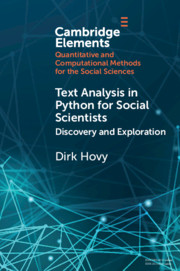
\includegraphics[width=.95\linewidth]{Sillabo/images/TextAnalysisInPythonForSocialScientists.jpg}
\end{minipage}\hfill
\begin{minipage}[b]{0.75\linewidth}          
	\noindent \textbf{Titolo:} Text Analysis in Python for Social Scientists - Discovery and Exploration \\
	\textbf{Autore:} Dirk Hovy \\
	\textbf{Casa editrice:} Cambridge University Press, publication year: 2021  \\
	\textbf{ISBN Online:} 9781108873352\\   
	\vspace{1cm}
	~
\end{minipage}
\vspace{.18cm}
\hrule
\vspace{.4cm}
\begin{minipage}[b]{0.17\linewidth}          
	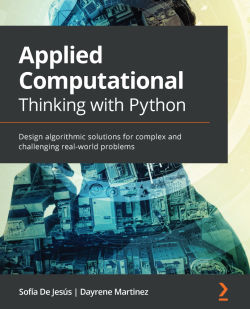
\includegraphics[width=.95\linewidth]{Sillabo/images/AppliedComputationalThinkingWithPython.jpeg}
\end{minipage}\hfill
\begin{minipage}[b]{0.75\linewidth}          
	\noindent \textbf{Titolo:} Applied Computational Thinking with Python \\
	\textbf{Autore:} Sof\'{i}a De Jes\'{u}s , Dayrene Martinez \\
	\textbf{Casa editrice:} Packt Publishing; publication year: 2020  \\
	\textbf{ISBN-13:} 978-1839219436\\  
	\vspace{1cm}
	~
\end{minipage}
\vspace{.18cm}
\hrule
\vspace{.4cm}
\begin{minipage}[t]{0.17\linewidth}          
	
\includegraphics[trim={0 0 0 1cm},clip, width=.95\linewidth,]{Sillabo/images/1200px-Wikibooks-logo.png}
\end{minipage}\hfill
\begin{minipage}[b]{0.75\linewidth}  
    \vspace{.5cm}
	\noindent \textbf{Titolo:} The LaTeX Wikibook  \\
	\textbf{Autore:} Multipli \\
	\textbf{Casa editrice:} Wikibooks community  \\
	\textbf{Disponibile online:} \url{https://en.wikibooks.org/wiki/LaTeX}\\
	\vspace{1cm}
	~
\end{minipage}
\vspace{.18cm}
\hrule

\\

%--------  Required Software and Material ------------------------------
\vspace{.4cm}

\customsection{Strumenti software utilizzati }  
\begin{itemize}[itemsep=2pt,parsep=0pt,topsep=2pt,partopsep=2pt]
	%    \item[\color{darkblue}\faCoffee] Java 7 or 8 (32 or 64 bits)
	\item[\color{darkblue}\faLaptopCode] \textbf{Sistemi operativi:} \faWindows {} Windows  10,  \faLinux {} Linux, \textcolor{vanierred}{\textbf{o}} \faApple {} macOS 
	\item[\color{darkblue}\faCode] \textbf{IDE per Python:} \faUnity a scelta dello studente, da coordinare con il parallelo corso di laboratorio di programmazione
	\item [{\color{darkblue}\faChrome}] \textbf{Web Browser:} Chrome, Safari o Firefox.   
	\item[{\color{darkblue} \faWpforms}] LaTex per la produzione e l'analisi di documenti; all'uopo gli studenti sono incoraggiati a crearsi un account su \url{overleaf.com} e comunicarlo al docente
\end{itemize}   

\customsection{Regole di comportamento} 
\begin{itemize}[itemsep=2.5pt,parsep=0pt,topsep=8pt,partopsep=4pt]
	\item[{ \color{darkblue} \faLaptop \faMobile \faHeadphones}] In classe, l'uso di cellulari, di computer e di cuffie, quando non richiesto dal docente, \`{e}  \underline{vietato}. I cellulari vanno spenti e riposti in luogo sicuro non nei banchi.
	
	\item[{\color{darkblue} \faEdit}] Il docente si aspetta che gli studenti si presentino con carta e penna/matita e prendano attivamente appunti.
	\item[{\color{darkblue} \faWechat}] Gli studenti sono ammessi alle lezioni solo all'inizio e durante le lezioni devono astenersi dal parlare tra loro, se non quando esplicitamente richiesto dal docente.
	
	\item[{\color{darkred} \faThumbsDown}] Il plagiarismo negli elaborati comporter\`{a} la bocciatura nell'esame e le ulteriori penalit\`{a} previste nei competenti regolamenti accademici.
\end{itemize}


\customsection{Programma di massima delle lezioni}
\newcounter{lezione}
\setcounter{lezione}{0}
\addtocounter{lezione}{1}

%TODO: split implementation into 3 builds.
\renewcommand{\arraystretch}{1.5} % this reduces the vertical spacing between rows    
\noindent\begin{longtable}{|C{1cm}|p{15cm}|}
\toprule
	\thead{\color{darkblue} Lezione} & \thead{\argomento, \materialedidattico \& \dataeora} \\ 
	%---s Load the table body: dynamic table content. 
\midrule
    \endhead
	\centering\textbf{\thelezione \addtocounter{lezione}{1}} &   \argomento[Presentazione del corso e natura del mercato e del dato]  \\
	& \materialedidattico[\href{https://github.com/GiancarloSucci/UniBo.IDSEPC.A2022/blob/main/A2022.IDSEPCL03.L04.pdf}{Lucidi presentati dal docente sul corso e sulla natura del mercato e del dato}] \\
	& \dataeora[20 settembre 2022, 18-20] \\
	\hline    
	\centering\textbf{\thelezione \addtocounter{lezione}{1}} &   \argomento[La produzione del dato nel lavoro (condiviso); gitHub]  \\
	& \materialedidattico[Lucidi presentati dal docente] \\
	& \dataeora[21 settembre 2022, 16-18] \\
	\hline    
	\centering\textbf{\thelezione \addtocounter{lezione}{1}} &   \argomento[Il dato come documento; La scrittura di documenti in LaTex come paradigma della produzione digitale (parte 1)]  \\
	& \materialedidattico[\href{https://github.com/GiancarloSucci/UniBo.IDSEPC.A2022/blob/main/A2022.IDSEPCL03.L04.pdf}{Lucidi presentati dal docente su LaTeX}] \\
	& \dataeora[21 settembre 2022, 18-20] \\
	\hline    
	\centering\textbf{\thelezione \addtocounter{lezione}{1}} &   \argomento[La scrittura di documenti in LaTex come paradigma della produzione digitale (parte 2)]  \\
	& \materialedidattico[\href{https://github.com/GiancarloSucci/UniBo.IDSEPC.A2022/blob/main/A2022.IDSEPCL03.L04.pdf}{Lucidi presentati dal docente su LaTeX}] \\
	& \dataeora[5 ottobre 2022, 16-18] \\
	\hline    
%	\textbf{\thelezione \addtocounter{lezione}{1}} &   \argomento[Struttura dei calcolatori]  \\
%	& \materialedidattico \\
%	\hline    
%	\textbf{\thelezione \addtocounter{lezione}{1}} &   \argomento[Sistemi operativi e reti]  \\
%	& \materialedidattico \\
%	\hline    
%	\textbf{\thelezione \addtocounter{lezione}{1}} &   \argomento[Linguaggi di programmazione]  \\
%	& \materialedidattico \\
%	\hline    
	\textbf{\thelezione \addtocounter{lezione}{1}} &   \argomento[Processo di produzione del software]  \\
	& \materialedidattico \\
	& \dataeora[5 ottobre 2022, 18-20] \\
	\hline    
	\textbf{\thelezione \addtocounter{lezione}{1}} &   \argomento[Sperimentazione e deduzione; il modello GQM]  \\
	& \materialedidattico \\
	& \dataeora[11 ottobre 2022, 18-20, 18-20] \\
	\hline    
	\textbf{\thelezione \addtocounter{lezione}{1}} &   \argomento[Scale di dati]  \\
	& \materialedidattico \\
	& \dataeora[12 ottobre 2022, 16-18] \\
	\hline    
	\textbf{\thelezione \addtocounter{lezione}{1}} &   \argomento[Revisione dei fondamenti di statistica descrittiva (parte 1)]  \\
	& \materialedidattico \\
	& \dataeora[12 ottobre 2022, 18-20] \\
	\hline    
	\textbf{\thelezione \addtocounter{lezione}{1}} &   \argomento[Revisione dei fondamenti di statistica descrittiva (parte 2)]  \\
	& \materialedidattico \\
	& \dataeora[18 ottobre 2022, 18-20] \\
	\hline    
	\textbf{\thelezione \addtocounter{lezione}{1}} &   \argomento[Progettazione degli esperimenti]  \\
	& \materialedidattico \\
	& \dataeora[19 ottobre 2022, 16-18] \\
	\hline    
	\textbf{\thelezione \addtocounter{lezione}{1}} &   \argomento[Statistica inferenziale -- le basi e principi di regressione lineare]  \\
	& \materialedidattico \\
	& \dataeora[19 ottobre 2022, 18-20] \\
	\hline
	\textbf{\thelezione \addtocounter{lezione}{1}} &   \argomento[Statistica inferenziale -- regressione lineare]  \\
& \materialedidattico \\
	& \dataeora[8 novembre 2022, 18-20] \\
	\hline
	\textbf{\thelezione \addtocounter{lezione}{1}} &   \argomento[Statistica inferenziale -- la correlazione parametrica]  \\
& \materialedidattico \\
	& \dataeora[9 novembre 2022, 16-18] \\
	\hline
	\textbf{\thelezione \addtocounter{lezione}{1}} &   \argomento[Dalla statistica inferenziale all’apprendimento automatico; la regressione logistica]  \\

   & \materialedidattico \\
	& \dataeora[9 novembre 2022, 18-20] \\
	\hline    
   \textbf{\thelezione \addtocounter{lezione}{1}} &   \argomento[Principi di reti neurali (parte 1)]  \\
	& \materialedidattico \\
	& \dataeora[15 novembre 2022, 18-20] \\
	\hline    
	\textbf{\thelezione \addtocounter{lezione}{1}} &   \argomento[Principi di reti neurali (parte 2)]  \\
	& \materialedidattico \\
	& \dataeora[16 novembre 2022, 16-18] \\
	\hline    
	\textbf{\thelezione \addtocounter{lezione}{1}} &   \argomento[Principi di reti neurali (parte 3)]  \\
	& \materialedidattico \\
	& \dataeora[16 novembre 2022, 18-20] \\
	\hline    
	\textbf{\thelezione \addtocounter{lezione}{1}} &   \argomento[Analisi automatica di testi (parte 1)]  \\
	& \materialedidattico \\
	& \dataeora[23 novembre 2022, 18-20] \\
	\hline    
	\textbf{\thelezione \addtocounter{lezione}{1}} &   \argomento[Analisi automatica di testi (parte 2)]  \\
	& \materialedidattico \\
	& \dataeora[29 novembre 2022, 18-20] \\
	\hline    
	\textbf{\thelezione \addtocounter{lezione}{1}} &   \argomento[Analisi automatica di testi (parte 3)]  \\
	& \materialedidattico \\
	& \dataeora[30 novembre 2022, 18-20] \\
	\hline    

\end{longtable}   

\vspace{1cm}
\noindent \textcolor{red}{\textbf{\underline{NOTA:}}} Il programma sopra specificato pu\`{o} essere modificato per esigenze organizzative e didattiche. 

\end{document} 